\nomenclature[]{MLE}{Maximum Likelihood Estimate}
\note{Make sure it's clear whether using random variables or not}
\note{Might need to make clear Markov assumptions }
As discussed, HMMs and DBNs are useful tools for modelling complex random dynamic processes. Typically, models are used to provide some kind of inference about a process, to gain insight into its inner workings. By inference, we mean calculating the probability distributions over variables of interest. Some algorithms will be outlined here that will demonstrate how to calculate both exact and approximate inferences, using general structures for HMMs and DBNs. \par

First, inference algorithms commonly used with HMMs are discussed, as their representation is more rigid, meaning that it is easier to exploit their structure generally to perform inference. As previously stated, HMMs and DBNs are routinely used to model systems that have state variables that cannot be directly observed. In most cases, we are interested in inferring what the state of the system might be, given the observed evidence variables received. This is the first and arguably the most useful inference challenge that we inspect.

The actual quantity that we want to compute is 
\[P(X_t | e_1, e_2, ..., e_t) = P(X_t | e_{1:t})\]
that is, the probability distribution of the hidden state variable, given all previously observed evidence variables. The notation $e_{1:t}$ denotes the joint distribution of $e_1, e_2, ..., e_t$ This is the \textit{filtering} problem, mentioned in section \ref{Chapter:HMM}. We are interested in computing this value, rather than the unconditional state distribution, $P(X_t)$, because .... \note{Explain this carefully}.The conditional distribution $P(X_t | e_{1:t})$ is frequently referred to as the \textit{belief state} and the process of calculation of this distribution is frequently referred to as \textit{state estimation} or \textit{filtering}. The \textit{forward algorithm} is frequently used to calculate the value of $P(X_t | e_{1:t})$. It is a recursive algorithm, and takes advantage of the fact that the underlying process is Markovian. The well-known forward algorithm for HMMs is shown in algorithm \ref{alg:bayes_filter_observations_only}. The derivation is useful to follow as an exercise:
\subsubsection{HMM Filtering Algorithm Derivation} 
\label{section:HMMFiltering}
\note{Might be better to put this in an appendix.}
Two well-known probability identities are used in the derivation: 
\note{Fix the formatting here}
\begin{center}
- - - - - - - - - - - - - - - - - - - - - - - - - - - - - - - - - - - - - - - - - - - - - - - - - - - - - - - - - - - - - 
\end{center}
%quad adds space
\[(a) \quad p(A | B, C) = \frac{p(B | A, C) p(A | C)}{p(B | C)} \quad \text{and} \quad (b) \quad p(A | B) = \int\limits_{C}P(A | B, C) P(C | B)dC\]

\begin{center}
- - - - - - - - - - - - - - - - - - - - - - - - - - - - - - - - - - - - - - - - - - - - - - - - - - - - - - - - - - - - - 
\end{center}

\begin{enumerate}
\item {\hfil $ p(x_t | e_{1:t}) = p(x_t | e_{1:t-1}, e_t) $ }

\item {\hfil $ \text{applying (a) and letting} \quad \eta = \frac{1}{p(e_t | e_{1:t-1})} \quad = \quad \eta p(e_t | e_{1:t-1}, x_t)p(x_t|e_{1:t-1}) $ }

\item {\hfil $ \text{by the Markov property} \quad = \quad \eta p(e_t | x_t)p(x_t|e_{1:t-1})$}

\item {\hfil $\text{applying (b)} \quad =  \quad \eta p(e_t | X_t)\int_{x_{t-1}}p(x_t|e_{1:t-1}, x_{t-1}) p(x_{t-1}|e_{1:t-1})dx_{t-1}$}

\item {\hfil  $ \text{by the Markov property} \quad = \quad \eta p(e_t | x_t)\int_{x_{t-1}}p(x_t|x_{t-1}) p(x_{t-1}|e_{1:t-1})dx_{t-1} $}

\end{enumerate}
Note that $\eta$ is a normalizing constant that ensures that the probability distribution integrates to 1, and that the probabilities that need to be calculated can be done so from the parameters specified in the HMM; namely $p(e_t | X_t)$, specified by the sensor model, and $p(X_t | x_{t-1})$, specified by the transition model.

\begin{algorithm}{}
\caption{Forward Algorithm for HMMs}
\label{alg:bayes_filter_observations_only}

\begin{algorithmic}[1]
\renewcommand{\algorithmicrequire}{\textbf{Input:}}
\renewcommand{\algorithmicensure}{\textbf{Output:}}
%Input
\REQUIRE $\newline P(x_{t-1} | e_{1:t-1})=bel(x_{t-1}), \text{ the belief distribution as far as the previous timestep}
\newline e_t, \text{ the most recent observation}
\newline hmm, \text{(a Hidden Markov Model specifying the transition and observation probabilities}$
%Output
\ENSURE  $\newline P(X_{t} | e_{1:t}) = bel(X_{t})$

\hfill\pagebreak

\FOR{all $x_t$}
\STATE $\overline{bel}(x_t) = \int p(X_t | x_{t-1}) p(X_{t-1} | e_{1:t-1}) d x_{t-1}$
\STATE $bel(x_t) = p(e_t | x_t) \overline{bel}(x_t)$
\ENDFOR
\STATE $ \eta = 1 / \int_{x_t}{bel(x_t)}dx_t$
 \FOR{all $x_t$ do:}
\STATE $bel(x_t) = \eta{bel}(x_t)$
\ENDFOR  
    
%\WHILE {pointsToVisit is not empty}

%\STATE agentPosition $\leftarrow$ last value in agentPaths.get(agent)

%\STATE P$\leftarrow$\(\displaystyle \min_{p \in pointsToVisit}\)cost(agentPosition, p)

%\STATE Update currentAgent value in AgentPaths to include P
%\STATE Add P to visitedPoints.
%\STATE Remove P from pointsToVisit.
%\STATE currentAgentIndex$\leftarrow$(currentAgentIndex+1) $\mathbf{mod}$$\vert$List of Agents$\vert$
%\STATE currentAgent$\leftarrow$agents.get(currentAgentIndex)


%\ENDWHILE
\RETURN $bel(X_t)$
\end{algorithmic} 
\end{algorithm}

\note{Don't forget to mention: Sufficient statistics, forward algorithm}

Algorithm \ref{alg:bayes_filter_observations_only} uses integrals to account for the fact that the distribution being used may be continuous. The work done in this thesis only uses discrete distributions, and so summations are used instead of integrals for the subsequent discussion. A consequence of using discrete distributions is that it is possible to formulate the forward algorithm using vector and matrix notation. As outlined in section \ref{Chapter:HMM}, the transition model for a HMM can be written down in matrix form, as can the observation model. This allows for a highly compact notation: denoting $p(x_t | e_{1:t})$ as $f_{1:t}$, we can write $f_{1:t} = \eta O_{t} T^{T} f_{1:t-1}$, where $f_{1:t}$ contains the vector of values of $p(x_t | e_{1:t})$ for every possible $x_t$ \cite[p.~579]{AIAMA}. Note that the observation model, $O_t$ is time dependent, as opposed to the transition model, which is assumed to be stationary.\par

Some insight can be gained from studying Algorithm \ref{alg:bayes_filter_observations_only}. There are three main steps to this algorithm, and the intuition behind them is explained: 
\note{These are highly verbose, edit to make less wordy}
\begin{enumerate}
    
    \item The first step is often referred to as the prediction step:
    \begin{center}
    $\overline{bel}(x_t) = \sum_{x_{t-1}} p(x_t | x_{t-1}) p(x_{t-1} | e_{1:t-1}) d x_{t-1}$
    \end{center}

    This step carries out the first part of the calculation of the belief value for a given state $x_t$, by marginalizing over all possible hidden states ($x_{t-1}$) that could have preceded the current one ($x_t$). This is highly intuitive; the probability of being in state $x_t$ should depend on the probability of transitioning from all possible previous states to $x_t$. 
    \note{this sentence doesn't seem necessary}
    Think "\textit{the probability that I am in location x is the sum of probabilities of starting at all other possible locations and subsequently ending up in location x, weighted against my belief that I began in each other possible location}".
    
    %product of our most recent belief of being in state $x_{t-1}$, given by $p(x_{t-1} | e_{1:t-1})$ and the probability of transitioning from that state to state $x_{t}$, for all previous possible states that we could have been in. 
    $\overline{bel}(x_t)$ effectively projects our current belief to the next time step by using the transition probabilities specified in the HMM.
    
    \item The second step is often referred to as the correction step, or the measurement update step: 
    \begin{center}
    $bel(x_t) = p(e_t | x_t) \overline{bel}(x_t)$ 
    \end{center}
    This step takes the projected belief in step 1 and multiplies it by the probability of observing the data that we did in the given hidden state, $x_t$. This can be thought of as a correction because the use of the measurement data narrows down the possible states that the system could be in. 
    \note{Need to re-word this to make more concise}
    For example, if the value of a transition probability from state x to state y is low, and there is a low probability that the system was previously in state x, a high probability of observing the observed sensor reading given state y can still result in a high posterior probability of the system being in state y given the new evidence.
    
    \item The final step is to ensure that the distribution sums to 1. This is done by multiplying by a normalizing constant, $\eta$.
    
    
\end{enumerate}
It is also worth noting that algorithm \ref{alg:bayes_filter_observations_only} is recursive, meaning that updates can be performed online. This means that an agent can iteratively update its estimated state (or belief) as new percepts are recorded. Also note that an initial distribution of the estimated state must be provided to this algorithm before updated can be performed. The complexity of the forward algorithm is $\theta (nm^2)$, where m is the size of the joint distribution of the hidden variables, x, and n is the number of timesteps that have occurred. This is clear to see when viewing the update as the matrix-vector multiplication $f_{1:t} = \eta O_{t} T^{T} f_{1:t-1}$, as the size of T is $m^2$.






\subsubsection{Evidence Likelihood Algorithm Using a HMM}
\note{Will talk about this briefly for SPRT}
The second useful quantity that we would like to calculate is the probability of observing the evidence that we did, often referred to the likelihood function of the data, as identified in section \ref{Chapter:HMM}. In simpler terms, this means we calculate the probability of observing the data, given a fixed parameterised model of the data (the HMM). This value is useful as it can reveal insights into whether one model is more likely than another model, with applications including \textbf{M}aximum \textbf{a} \textbf{P}osteriori (MAP) parameter estimates and hypothesis testing. We would like to compute the value of
\[P(e_1, e_2, ..., e_t) = P(e_{1:t})\]
given the fixed set of parameters provided by the HMM. A brief outline of the derivation provided in ... .\note{Put the derivation in an appendix} The derivation clearly shows that the algorithm for calculating likelihoods is exactly the same as forward algorithm, with the replacement of  $p(x_{t-1}|e_{1:t-1})$ with $p(x_t-1, e_{1:t-1})$ and one final summation.


\subsubsection{HMM Evidence Likelihood Algorithm Derivation}\label{section:EvidenceLikelihood}

Analagous to ..., two well-known probability identities are used in the derivation: 
\begin{center}
- - - - - - - - - - - - - - - - - - - - - - - - - - - - - - - - - - - - - - - - - - - - - - - - - - - - - - - - - - - - - 
\end{center}
%quad adds space
\[(a) \quad p(A, B, C) = p(A | B, C) p(B, C) \quad \text{and} \quad (b) \quad p(A, B) = \sum_{C}{p(A | B, C)p(B, C)}\]

\begin{center}
- - - - - - - - - - - - - - - - - - - - - - - - - - - - - - - - - - - - - - - - - - - - - - - - - - - - - - - - - - - - - 
\end{center}


\begin{enumerate}

\item {\hfil $p(e_{1:t}) = \sum_{x_t}p(e_{1:t}, x_t) \quad = \quad \sum_{x_t}p({e_{1:t-1}, e_t, x_t}) $
}
\item {\hfil $\text{applying (a) } \quad= \quad
\sum_{x_t}{p(e_t | e_{1:t-1}, x_t)p(x_t, e_{1:t-1})}$
}
\item {\hfil $\quad \text{by the Markov property} 
\quad = \quad \sum_{x_t}p(e_t | x_t)p(x_t, e_{1:t-1})$
}

\item {\hfil $\text{applying (b)} \quad =  \quad
\sum_{x_t}p(e_t | x_t) \sum_{x_{t-1}}p(x_t|e_{1:t-1}, x_{t-1}) p(x_{t-1},e_{1:t-1})$
}

\item {\hfil $\text{by the Markov property} \quad = \quad 
\sum_{x_t}{p(e_t | x_t)\sum_{x_{t-1}}p(x_t|x_{t-1}) p(x_{t-1},e_{1:t-1})}$
}

\end{enumerate}

%No point in writing up likelihood algorithm as it's very similar to forward algorithm.

\subsubsection{HMM Parameter Learning Using Expectation Maximization}
\note{Can talk about this briefly for battery model}
Since a HMM is a parameterised model of a stochastic process, a natural question to ask is whether it is possible to determine a \textit{"best"} set of parameters to describe the process, by using observations of the process. This is a more complex version of the well-known process of finding the parameters that maximize the likelihood function of fully observable data, known as the \textbf{M}aximum \textbf{L}ikelihood \textbf{E}stimate (MLE). Finding the most likely set of parameters which provided the observed values can be described mathematically as the value of \note{fix argmax notation}$\argmax_{\lambda} P(E_{1:t} | \lambda)$. Note that this is a fundamentally different problem to that discussed in the preceding section; here we do not assume a fixed set of parameters for the HMM ($\lambda$).

This is a well-studied problem for HMMs and the solution is given by the \textbf{E}xpectation \textbf{M}aximisation (EM) algorithm, proposed by \citeauthor{Dempster1977MaximumAlgorithm}. This algorithm is reasonably complex and highly detailed overviews can be found in many texts that deal with parameter estimation for statistical models. A quick outline of how the algorithm works is provided here.\par


The reason why the standard methods for finding the MLE for a parameterised model do not work with HMMs is due to the fact that there is no way to directly express the quantity  $P(E_{1:t} | \lambda)$ directly. This can be seen in the derivation of the evidence likelihood in <reference whichever appendix it ends up in>. Instead, it is necessary to marginalize over states: $ P(e_{1:t} | \lambda) = \sum_{x_t}{p(x_t, e_{e:t} | \lambda)}$. The standard approach to finding the parameters that maximize a model is to take a log transform of the likelihood function, which preserves the solution but turns the problem into one of finding the parameters that maximize a sum rather than a product. Using standard methods of calculus, this can usually be done easily. The issue with HMMs is that when a logarithmic transformation is applied to the likelihood function, the summation sign remains within the log function, which means finding the maximum is still a difficult problem. The EM algorithm, taking the approach of many iterative techniques, relaxes the constraints on the problem in order to find a lower bound of the log-likelihood and then iteratively improves this lower bound with increasing likelihood values. 


The Baum-Welch algorithm is a special case of the EM algorithm and is frequently used to solve the problem of estimating the parameters of a HMM. The algorithm is described fully in appendix <reference appendix>.

















\subsubsection{Filtering Algorithm for DBNs}
\note{Extend HMM to add control variable}
\begin{wrapfigure}{r}{0.65\linewidth}
    \centering
    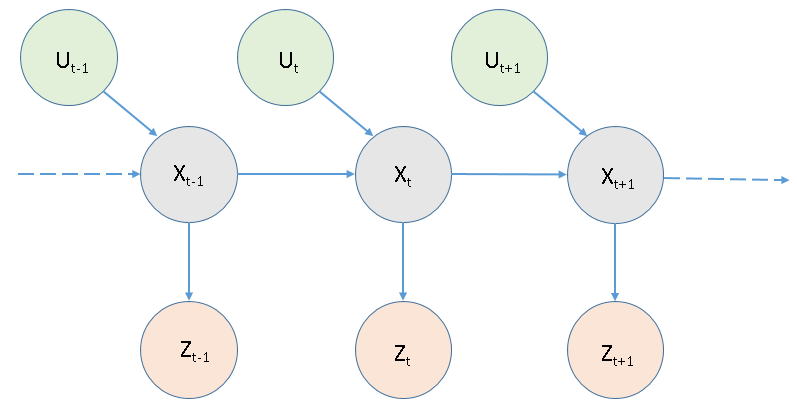
\includegraphics[width = 0.65\linewidth]{Chapters/MultiAgentTargetDetection/BayesianFiltering/Figs/HMMs/HMMWithControl.png}
    \caption{A DBN with Hidden State variables (grey), Observation variables (orange) and Control variables (green).}
    \label{fig:HMMWithControlVariablesExample}
\end{wrapfigure}
The forward algorithm for \textit{state estimation}, or \textit{filtering} was presented in section \ref{section:HMMFiltering}. A slightly modified version of this algorithm is now described, which is very commonly used in stochastic systems that can be influenced by actions that an agent may take. Such systems have \textit{control variables} as well as hidden state variables and observation variables. These control variables (variables which represent the actions that an agent may perform) have an influence on the transition probabilities between states. The graphical model in figure \ref{fig:HMMWithControlVariablesExample} describes the basic case. The arrows describe the conditional independence assumptions: at time t, the hidden state ($x_t$) depends on the previous state ($x_{t-1}$), and the previous control action taken ($u_t$). As with the HMM, the observation $e_t$ is conditionally dependent on the state $x_t$. This causes a slight change in the filtering algorithm: on line 2 of algorithm \ref{alg:bayes_filter_observations_only}: $\overline{bel}(x_t) = \sum_{x_{t-1}} p(x_t | x_{t-1}) p(x_{t-1} | e_{1:t-1}) $ is replaced with $\overline{bel}(x_t) = \sum_{x_{t-1}} p(x_t | u_t, x_{t-1}) p(x_{t-1} | e_{1:t-1}, u_{1:t-1}) $, which is intuitive: transition probabilities now depend on the most recent control action taken, as well as the previous state.


%DBNs have already been shown to be a powerful tool while modelling stochastic systems, since the hidden variables can be described by conditional independences, rather than 



This algorithm can be further generalized - if multiple control variables, hidden state variables and observation variables are needed to describe the system fully, it is possible to make minor modifications which reflect the conditional independences stated by the underlying DBN. It is also worth noting that there are many well-known filtering algorithms that deal with data that come from certain distributions and satisfy constraints related to their transition and observation models, for example the Kalman Filter.






%\subsubsection{Discrete Bayes Filter}
%\note{This is what is used in the work that I did, so it is outlined}

\subsubsection{Approximate State Estimation Algorithms}
\note{Thought about using Particle filter to avoid the dimensionality problem when attempting to maintain estimated state}
The state estimation algorithms mentioned so far maintain the exact values of the distribution $p(x_t | e_{1:t}, u_{1:t})$, but we will quickly mention some approximate methods that are also frequently used. The computational complexity of the general DBN updating algorithms is determined by how well the joint distribution of hidden state variables, observation variables and control action variables can be factored, but in the worst case the complexity is given by $O(n^2um)$, where n are the number of hidden states, u is the number of available control actions and m is the number of time steps. In some cases, this can become intractable, especially if the state space is large and the transition model cannot be efficiently factored. In this case, approximate techniques are used. By far the most common example is the \textit{particle filter}. For reference, the particle filter algorithm is provided in appendix <reference the appendix>. We will briefly discuss how the algorithm works here (P. 97 Thrun).

\note{Not sure if it's worth filling out this section further, since this gives a lot of the background for the subsequent discussion}